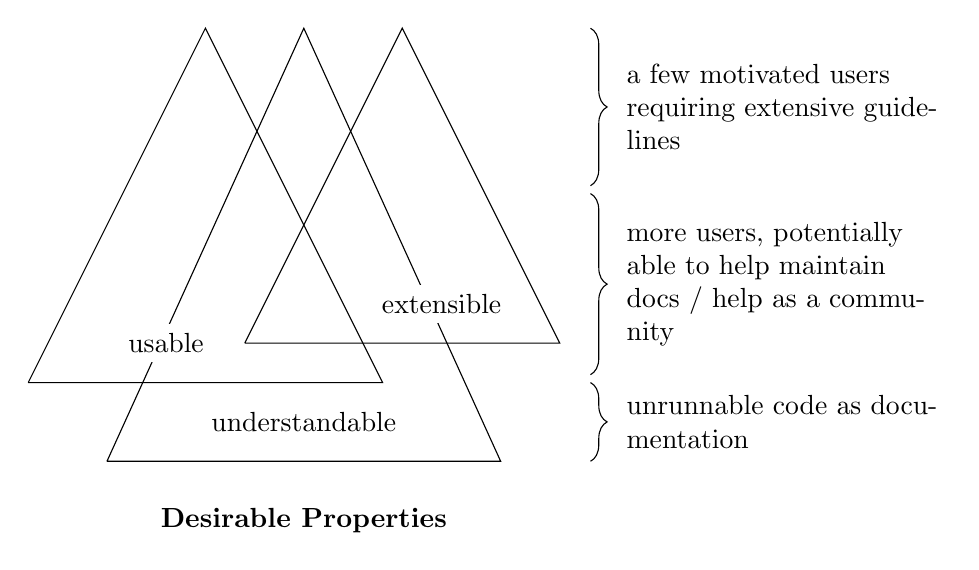
\begin{tikzpicture}

\def\h{5.5}
\def\noteOffsetY{3.5}

\coordinate (A1) at (-2.5, 0);
\coordinate (B1) at (   0, \h);
\coordinate (C1) at ( 2.5, 0);

\coordinate (A2) at (-3.5, 1);
\coordinate (B2) at (-1.25, \h);
\coordinate (C2) at ( 1.0, 1);

\coordinate (A3) at (-0.75, 1.5);
\coordinate (B3) at ( 1.25, \h);
\coordinate (C3) at ( 3.25, 1.5);

\draw[] (A1) -- (B1) -- (C1) -- (A1);
\draw[] (A2) -- (B2) -- (C2) -- (A2);
\draw[] (A3) -- (B3) -- (C3) -- (A3);

% triangle captions
\node(P1)[text centered, fill=white] at (-1.75,1.5) {usable};
\node(P2)[text centered, fill=white] at (1.75,2.0) {extensible};
\node(P3)[text centered, fill=white] at (0,0.5) {understandable};

\node(P4)[text centered, fill=white] at (0,-0.75) {\bf Desirable Properties};

\node(O)[text centered, scale=2] at (0,2) {$\bigstar$};

% sidenotes
\tikzstyle{bracestyleMirror}=[decorate,decoration={brace,amplitude=6pt,mirror,raise=4pt},yshift=0pt]
\tikzstyle{notestyle}=[black,midway,xshift=2.6cm, text width = 4cm]

\draw [style = bracestyleMirror] (\noteOffsetY,3.5) -- (\noteOffsetY,\h) node [style = notestyle] 
{a few motivated users requiring extensive guidelines};

\draw [style = bracestyleMirror] (\noteOffsetY,1.1) -- (\noteOffsetY,3.4) node [style = notestyle] 
{more users, potentially able to help maintain docs / help as a community};

\draw [style = bracestyleMirror] (\noteOffsetY,0) -- (\noteOffsetY,1) node [style = notestyle] 
{unrunnable code as documentation};

\end{tikzpicture}